% Created by tikzDevice version 0.10.1 on 2019-04-12 20:09:04
% !TEX encoding = UTF-8 Unicode
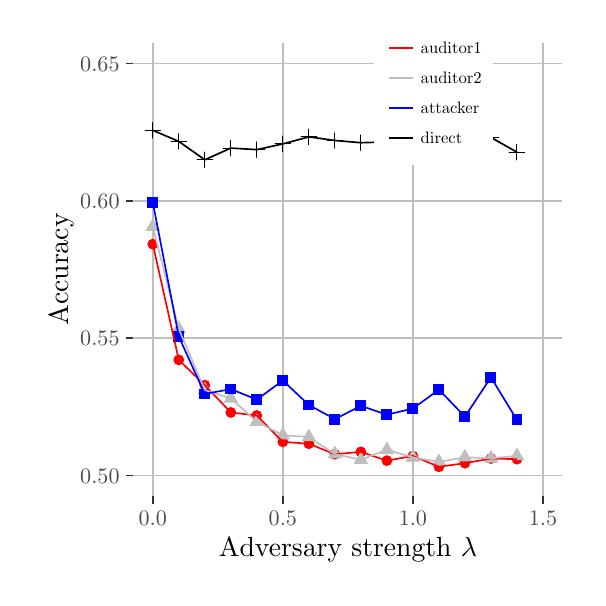
\begin{tikzpicture}[x=1pt,y=1pt]
\definecolor{fillColor}{RGB}{255,255,255}
\path[use as bounding box,fill=fillColor,fill opacity=0.00] (0,0) rectangle (198.74,198.74);
\begin{scope}
\path[clip] (  0.00,  0.00) rectangle (198.74,198.74);
\definecolor{drawColor}{RGB}{255,255,255}
\definecolor{fillColor}{RGB}{255,255,255}

\path[draw=drawColor,line width= 0.6pt,line join=round,line cap=round,fill=fillColor] ( -0.00,  0.00) rectangle (198.74,198.74);
\end{scope}
\begin{scope}
\path[clip] ( 38.16, 29.45) rectangle (193.24,193.24);
\definecolor{drawColor}{RGB}{255,255,255}

\path[draw=drawColor,line width= 0.3pt,line join=round] ( 38.16, 61.71) --
	(193.24, 61.71);

\path[draw=drawColor,line width= 0.3pt,line join=round] ( 38.16,111.34) --
	(193.24,111.34);

\path[draw=drawColor,line width= 0.3pt,line join=round] ( 38.16,160.98) --
	(193.24,160.98);

\path[draw=drawColor,line width= 0.3pt,line join=round] ( 68.70, 29.45) --
	( 68.70,193.24);

\path[draw=drawColor,line width= 0.3pt,line join=round] (115.70, 29.45) --
	(115.70,193.24);

\path[draw=drawColor,line width= 0.3pt,line join=round] (162.70, 29.45) --
	(162.70,193.24);
\definecolor{drawColor}{RGB}{190,190,190}

\path[draw=drawColor,line width= 0.6pt,line join=round] ( 38.16, 36.89) --
	(193.24, 36.89);

\path[draw=drawColor,line width= 0.6pt,line join=round] ( 38.16, 86.53) --
	(193.24, 86.53);

\path[draw=drawColor,line width= 0.6pt,line join=round] ( 38.16,136.16) --
	(193.24,136.16);

\path[draw=drawColor,line width= 0.6pt,line join=round] ( 38.16,185.80) --
	(193.24,185.80);

\path[draw=drawColor,line width= 0.6pt,line join=round] ( 45.21, 29.45) --
	( 45.21,193.24);

\path[draw=drawColor,line width= 0.6pt,line join=round] ( 92.20, 29.45) --
	( 92.20,193.24);

\path[draw=drawColor,line width= 0.6pt,line join=round] (139.20, 29.45) --
	(139.20,193.24);

\path[draw=drawColor,line width= 0.6pt,line join=round] (186.19, 29.45) --
	(186.19,193.24);
\definecolor{fillColor}{RGB}{255,0,0}

\path[fill=fillColor] ( 45.21,120.52) circle (  1.96);
\definecolor{fillColor}{RGB}{190,190,190}

\path[fill=fillColor] ( 45.21,129.93) --
	( 47.85,125.35) --
	( 42.56,125.35) --
	cycle;
\definecolor{fillColor}{RGB}{0,0,255}

\path[fill=fillColor] ( 43.24,133.67) --
	( 47.17,133.67) --
	( 47.17,137.60) --
	( 43.24,137.60) --
	cycle;
\definecolor{drawColor}{RGB}{0,0,0}

\path[draw=drawColor,line width= 0.4pt,line join=round,line cap=round] ( 42.43,161.65) -- ( 47.98,161.65);

\path[draw=drawColor,line width= 0.4pt,line join=round,line cap=round] ( 45.21,158.88) -- ( 45.21,164.43);
\definecolor{fillColor}{RGB}{255,0,0}

\path[fill=fillColor] ( 54.60, 78.70) circle (  1.96);
\definecolor{fillColor}{RGB}{190,190,190}

\path[fill=fillColor] ( 54.60, 92.97) --
	( 57.25, 88.40) --
	( 51.96, 88.40) --
	cycle;
\definecolor{fillColor}{RGB}{0,0,255}

\path[fill=fillColor] ( 52.64, 85.18) --
	( 56.57, 85.18) --
	( 56.57, 89.10) --
	( 52.64, 89.10) --
	cycle;

\path[draw=drawColor,line width= 0.4pt,line join=round,line cap=round] ( 51.83,157.64) -- ( 57.38,157.64);

\path[draw=drawColor,line width= 0.4pt,line join=round,line cap=round] ( 54.60,154.86) -- ( 54.60,160.41);
\definecolor{fillColor}{RGB}{255,0,0}

\path[fill=fillColor] ( 64.00, 69.59) circle (  1.96);
\definecolor{fillColor}{RGB}{190,190,190}

\path[fill=fillColor] ( 64.00, 70.85) --
	( 66.65, 66.28) --
	( 61.36, 66.28) --
	cycle;
\definecolor{fillColor}{RGB}{0,0,255}

\path[fill=fillColor] ( 62.04, 64.41) --
	( 65.97, 64.41) --
	( 65.97, 68.33) --
	( 62.04, 68.33) --
	cycle;

\path[draw=drawColor,line width= 0.4pt,line join=round,line cap=round] ( 61.23,151.00) -- ( 66.78,151.00);

\path[draw=drawColor,line width= 0.4pt,line join=round,line cap=round] ( 64.00,148.22) -- ( 64.00,153.77);
\definecolor{fillColor}{RGB}{255,0,0}

\path[fill=fillColor] ( 73.40, 59.70) circle (  1.96);
\definecolor{fillColor}{RGB}{190,190,190}

\path[fill=fillColor] ( 73.40, 67.83) --
	( 76.05, 63.26) --
	( 70.76, 63.26) --
	cycle;
\definecolor{fillColor}{RGB}{0,0,255}

\path[fill=fillColor] ( 71.44, 66.19) --
	( 75.37, 66.19) --
	( 75.37, 70.11) --
	( 71.44, 70.11) --
	cycle;

\path[draw=drawColor,line width= 0.4pt,line join=round,line cap=round] ( 70.63,155.22) -- ( 76.18,155.22);

\path[draw=drawColor,line width= 0.4pt,line join=round,line cap=round] ( 73.40,152.45) -- ( 73.40,158.00);
\definecolor{fillColor}{RGB}{255,0,0}

\path[fill=fillColor] ( 82.80, 58.61) circle (  1.96);
\definecolor{fillColor}{RGB}{190,190,190}

\path[fill=fillColor] ( 82.80, 59.42) --
	( 85.44, 54.85) --
	( 80.16, 54.85) --
	cycle;
\definecolor{fillColor}{RGB}{0,0,255}

\path[fill=fillColor] ( 80.84, 62.38) --
	( 84.76, 62.38) --
	( 84.76, 66.30) --
	( 80.84, 66.30) --
	cycle;

\path[draw=drawColor,line width= 0.4pt,line join=round,line cap=round] ( 80.03,154.67) -- ( 85.58,154.67);

\path[draw=drawColor,line width= 0.4pt,line join=round,line cap=round] ( 82.80,151.89) -- ( 82.80,157.44);
\definecolor{fillColor}{RGB}{255,0,0}

\path[fill=fillColor] ( 92.20, 49.07) circle (  1.96);
\definecolor{fillColor}{RGB}{190,190,190}

\path[fill=fillColor] ( 92.20, 54.51) --
	( 94.84, 49.93) --
	( 89.56, 49.93) --
	cycle;
\definecolor{fillColor}{RGB}{0,0,255}

\path[fill=fillColor] ( 90.24, 69.28) --
	( 94.16, 69.28) --
	( 94.16, 73.20) --
	( 90.24, 73.20) --
	cycle;

\path[draw=drawColor,line width= 0.4pt,line join=round,line cap=round] ( 89.43,156.74) -- ( 94.98,156.74);

\path[draw=drawColor,line width= 0.4pt,line join=round,line cap=round] ( 92.20,153.97) -- ( 92.20,159.52);
\definecolor{fillColor}{RGB}{255,0,0}

\path[fill=fillColor] (101.60, 48.40) circle (  1.96);
\definecolor{fillColor}{RGB}{190,190,190}

\path[fill=fillColor] (101.60, 53.87) --
	(104.24, 49.30) --
	( 98.96, 49.30) --
	cycle;
\definecolor{fillColor}{RGB}{0,0,255}

\path[fill=fillColor] ( 99.64, 60.44) --
	(103.56, 60.44) --
	(103.56, 64.36) --
	( 99.64, 64.36) --
	cycle;

\path[draw=drawColor,line width= 0.4pt,line join=round,line cap=round] ( 98.83,159.28) -- (104.38,159.28);

\path[draw=drawColor,line width= 0.4pt,line join=round,line cap=round] (101.60,156.51) -- (101.60,162.06);
\definecolor{fillColor}{RGB}{255,0,0}

\path[fill=fillColor] (111.00, 44.60) circle (  1.96);
\definecolor{fillColor}{RGB}{190,190,190}

\path[fill=fillColor] (111.00, 47.69) --
	(113.64, 43.11) --
	(108.36, 43.11) --
	cycle;
\definecolor{fillColor}{RGB}{0,0,255}

\path[fill=fillColor] (109.04, 55.33) --
	(112.96, 55.33) --
	(112.96, 59.25) --
	(109.04, 59.25) --
	cycle;

\path[draw=drawColor,line width= 0.4pt,line join=round,line cap=round] (108.22,157.98) -- (113.77,157.98);

\path[draw=drawColor,line width= 0.4pt,line join=round,line cap=round] (111.00,155.20) -- (111.00,160.75);
\definecolor{fillColor}{RGB}{255,0,0}

\path[fill=fillColor] (120.40, 45.45) circle (  1.96);
\definecolor{fillColor}{RGB}{190,190,190}

\path[fill=fillColor] (120.40, 45.69) --
	(123.04, 41.11) --
	(117.76, 41.11) --
	cycle;
\definecolor{fillColor}{RGB}{0,0,255}

\path[fill=fillColor] (118.44, 60.12) --
	(122.36, 60.12) --
	(122.36, 64.04) --
	(118.44, 64.04) --
	cycle;

\path[draw=drawColor,line width= 0.4pt,line join=round,line cap=round] (117.62,157.17) -- (123.17,157.17);

\path[draw=drawColor,line width= 0.4pt,line join=round,line cap=round] (120.40,154.39) -- (120.40,159.94);
\definecolor{fillColor}{RGB}{255,0,0}

\path[fill=fillColor] (129.80, 42.28) circle (  1.96);
\definecolor{fillColor}{RGB}{190,190,190}

\path[fill=fillColor] (129.80, 49.25) --
	(132.44, 44.68) --
	(127.16, 44.68) --
	cycle;
\definecolor{fillColor}{RGB}{0,0,255}

\path[fill=fillColor] (127.84, 56.93) --
	(131.76, 56.93) --
	(131.76, 60.86) --
	(127.84, 60.86) --
	cycle;

\path[draw=drawColor,line width= 0.4pt,line join=round,line cap=round] (127.02,157.45) -- (132.57,157.45);

\path[draw=drawColor,line width= 0.4pt,line join=round,line cap=round] (129.80,154.67) -- (129.80,160.22);
\definecolor{fillColor}{RGB}{255,0,0}

\path[fill=fillColor] (139.20, 43.98) circle (  1.96);
\definecolor{fillColor}{RGB}{190,190,190}

\path[fill=fillColor] (139.20, 46.54) --
	(141.84, 41.96) --
	(136.55, 41.96) --
	cycle;
\definecolor{fillColor}{RGB}{0,0,255}

\path[fill=fillColor] (137.24, 59.15) --
	(141.16, 59.15) --
	(141.16, 63.07) --
	(137.24, 63.07) --
	cycle;

\path[draw=drawColor,line width= 0.4pt,line join=round,line cap=round] (136.42,158.06) -- (141.97,158.06);

\path[draw=drawColor,line width= 0.4pt,line join=round,line cap=round] (139.20,155.29) -- (139.20,160.84);
\definecolor{fillColor}{RGB}{255,0,0}

\path[fill=fillColor] (148.60, 40.07) circle (  1.96);
\definecolor{fillColor}{RGB}{190,190,190}

\path[fill=fillColor] (148.60, 44.87) --
	(151.24, 40.30) --
	(145.95, 40.30) --
	cycle;
\definecolor{fillColor}{RGB}{0,0,255}

\path[fill=fillColor] (146.63, 65.97) --
	(150.56, 65.97) --
	(150.56, 69.90) --
	(146.63, 69.90) --
	cycle;

\path[draw=drawColor,line width= 0.4pt,line join=round,line cap=round] (145.82,154.26) -- (151.37,154.26);

\path[draw=drawColor,line width= 0.4pt,line join=round,line cap=round] (148.60,151.49) -- (148.60,157.04);
\definecolor{fillColor}{RGB}{255,0,0}

\path[fill=fillColor] (158.00, 41.37) circle (  1.96);
\definecolor{fillColor}{RGB}{190,190,190}

\path[fill=fillColor] (158.00, 46.57) --
	(160.64, 42.00) --
	(155.35, 42.00) --
	cycle;
\definecolor{fillColor}{RGB}{0,0,255}

\path[fill=fillColor] (156.03, 56.22) --
	(159.96, 56.22) --
	(159.96, 60.14) --
	(156.03, 60.14) --
	cycle;

\path[draw=drawColor,line width= 0.4pt,line join=round,line cap=round] (155.22,154.83) -- (160.77,154.83);

\path[draw=drawColor,line width= 0.4pt,line join=round,line cap=round] (158.00,152.05) -- (158.00,157.60);
\definecolor{fillColor}{RGB}{255,0,0}

\path[fill=fillColor] (167.39, 43.04) circle (  1.96);
\definecolor{fillColor}{RGB}{190,190,190}

\path[fill=fillColor] (167.39, 46.17) --
	(170.04, 41.60) --
	(164.75, 41.60) --
	cycle;
\definecolor{fillColor}{RGB}{0,0,255}

\path[fill=fillColor] (165.43, 70.45) --
	(169.36, 70.45) --
	(169.36, 74.37) --
	(165.43, 74.37) --
	cycle;

\path[draw=drawColor,line width= 0.4pt,line join=round,line cap=round] (164.62,159.08) -- (170.17,159.08);

\path[draw=drawColor,line width= 0.4pt,line join=round,line cap=round] (167.39,156.31) -- (167.39,161.86);
\definecolor{fillColor}{RGB}{255,0,0}

\path[fill=fillColor] (176.79, 42.82) circle (  1.96);
\definecolor{fillColor}{RGB}{190,190,190}

\path[fill=fillColor] (176.79, 47.05) --
	(179.44, 42.47) --
	(174.15, 42.47) --
	cycle;
\definecolor{fillColor}{RGB}{0,0,255}

\path[fill=fillColor] (174.83, 55.04) --
	(178.76, 55.04) --
	(178.76, 58.96) --
	(174.83, 58.96) --
	cycle;

\path[draw=drawColor,line width= 0.4pt,line join=round,line cap=round] (174.02,153.76) -- (179.57,153.76);

\path[draw=drawColor,line width= 0.4pt,line join=round,line cap=round] (176.79,150.99) -- (176.79,156.54);
\definecolor{drawColor}{RGB}{255,0,0}

\path[draw=drawColor,line width= 0.6pt,line join=round] ( 45.21,120.52) --
	( 54.60, 78.70) --
	( 64.00, 69.59) --
	( 73.40, 59.70) --
	( 82.80, 58.61) --
	( 92.20, 49.07) --
	(101.60, 48.40) --
	(111.00, 44.60) --
	(120.40, 45.45) --
	(129.80, 42.28) --
	(139.20, 43.98) --
	(148.60, 40.07) --
	(158.00, 41.37) --
	(167.39, 43.04) --
	(176.79, 42.82);
\definecolor{drawColor}{RGB}{190,190,190}

\path[draw=drawColor,line width= 0.6pt,line join=round] ( 45.21,126.88) --
	( 54.60, 89.92) --
	( 64.00, 67.80) --
	( 73.40, 64.78) --
	( 82.80, 56.37) --
	( 92.20, 51.46) --
	(101.60, 50.82) --
	(111.00, 44.64) --
	(120.40, 42.64) --
	(129.80, 46.20) --
	(139.20, 43.49) --
	(148.60, 41.82) --
	(158.00, 43.52) --
	(167.39, 43.12) --
	(176.79, 43.99);
\definecolor{drawColor}{RGB}{0,0,255}

\path[draw=drawColor,line width= 0.6pt,line join=round] ( 45.21,135.64) --
	( 54.60, 87.14) --
	( 64.00, 66.37) --
	( 73.40, 68.15) --
	( 82.80, 64.34) --
	( 92.20, 71.24) --
	(101.60, 62.40) --
	(111.00, 57.29) --
	(120.40, 62.08) --
	(129.80, 58.90) --
	(139.20, 61.11) --
	(148.60, 67.94) --
	(158.00, 58.18) --
	(167.39, 72.41) --
	(176.79, 57.00);
\definecolor{drawColor}{RGB}{0,0,0}

\path[draw=drawColor,line width= 0.6pt,line join=round] ( 45.21,161.65) --
	( 54.60,157.64) --
	( 64.00,151.00) --
	( 73.40,155.22) --
	( 82.80,154.67) --
	( 92.20,156.74) --
	(101.60,159.28) --
	(111.00,157.98) --
	(120.40,157.17) --
	(129.80,157.45) --
	(139.20,158.06) --
	(148.60,154.26) --
	(158.00,154.83) --
	(167.39,159.08) --
	(176.79,153.76);
\end{scope}
\begin{scope}
\path[clip] (  0.00,  0.00) rectangle (198.74,198.74);
\definecolor{drawColor}{gray}{0.30}

\node[text=drawColor,anchor=base east,inner sep=0pt, outer sep=0pt, scale=  0.80] at ( 33.21, 34.14) {0.50};

\node[text=drawColor,anchor=base east,inner sep=0pt, outer sep=0pt, scale=  0.80] at ( 33.21, 83.77) {0.55};

\node[text=drawColor,anchor=base east,inner sep=0pt, outer sep=0pt, scale=  0.80] at ( 33.21,133.41) {0.60};

\node[text=drawColor,anchor=base east,inner sep=0pt, outer sep=0pt, scale=  0.80] at ( 33.21,183.04) {0.65};
\end{scope}
\begin{scope}
\path[clip] (  0.00,  0.00) rectangle (198.74,198.74);
\definecolor{drawColor}{gray}{0.20}

\path[draw=drawColor,line width= 0.6pt,line join=round] ( 35.41, 36.89) --
	( 38.16, 36.89);

\path[draw=drawColor,line width= 0.6pt,line join=round] ( 35.41, 86.53) --
	( 38.16, 86.53);

\path[draw=drawColor,line width= 0.6pt,line join=round] ( 35.41,136.16) --
	( 38.16,136.16);

\path[draw=drawColor,line width= 0.6pt,line join=round] ( 35.41,185.80) --
	( 38.16,185.80);
\end{scope}
\begin{scope}
\path[clip] (  0.00,  0.00) rectangle (198.74,198.74);
\definecolor{drawColor}{gray}{0.20}

\path[draw=drawColor,line width= 0.6pt,line join=round] ( 45.21, 26.70) --
	( 45.21, 29.45);

\path[draw=drawColor,line width= 0.6pt,line join=round] ( 92.20, 26.70) --
	( 92.20, 29.45);

\path[draw=drawColor,line width= 0.6pt,line join=round] (139.20, 26.70) --
	(139.20, 29.45);

\path[draw=drawColor,line width= 0.6pt,line join=round] (186.19, 26.70) --
	(186.19, 29.45);
\end{scope}
\begin{scope}
\path[clip] (  0.00,  0.00) rectangle (198.74,198.74);
\definecolor{drawColor}{gray}{0.30}

\node[text=drawColor,anchor=base,inner sep=0pt, outer sep=0pt, scale=  0.80] at ( 45.21, 18.99) {0.0};

\node[text=drawColor,anchor=base,inner sep=0pt, outer sep=0pt, scale=  0.80] at ( 92.20, 18.99) {0.5};

\node[text=drawColor,anchor=base,inner sep=0pt, outer sep=0pt, scale=  0.80] at (139.20, 18.99) {1.0};

\node[text=drawColor,anchor=base,inner sep=0pt, outer sep=0pt, scale=  0.80] at (186.19, 18.99) {1.5};
\end{scope}
\begin{scope}
\path[clip] (  0.00,  0.00) rectangle (198.74,198.74);
\definecolor{drawColor}{RGB}{0,0,0}

\node[text=drawColor,anchor=base,inner sep=0pt, outer sep=0pt, scale=  1.00] at (115.70,  7.70) {Adversary strength $\lambda$};
\end{scope}
\begin{scope}
\path[clip] (  0.00,  0.00) rectangle (198.74,198.74);
\definecolor{drawColor}{RGB}{0,0,0}

\node[text=drawColor,rotate= 90.00,anchor=base,inner sep=0pt, outer sep=0pt, scale=  1.00] at ( 14.59,111.34) {Accuracy};
\end{scope}
\begin{scope}
\path[clip] (  0.00,  0.00) rectangle (198.74,198.74);
\definecolor{fillColor}{RGB}{255,255,255}

\path[fill=fillColor] (125.12,149.11) rectangle (168.31,204.62);
\end{scope}
\begin{scope}
\path[clip] (  0.00,  0.00) rectangle (198.74,198.74);
\definecolor{drawColor}{RGB}{255,0,0}

\path[draw=drawColor,line width= 0.6pt,line join=round] (130.47,191.32) -- (139.14,191.32);
\end{scope}
\begin{scope}
\path[clip] (  0.00,  0.00) rectangle (198.74,198.74);
\definecolor{drawColor}{RGB}{190,190,190}

\path[draw=drawColor,line width= 0.6pt,line join=round] (130.47,180.48) -- (139.14,180.48);
\end{scope}
\begin{scope}
\path[clip] (  0.00,  0.00) rectangle (198.74,198.74);
\definecolor{drawColor}{RGB}{0,0,255}

\path[draw=drawColor,line width= 0.6pt,line join=round] (130.47,169.64) -- (139.14,169.64);
\end{scope}
\begin{scope}
\path[clip] (  0.00,  0.00) rectangle (198.74,198.74);
\definecolor{drawColor}{RGB}{0,0,0}

\path[draw=drawColor,line width= 0.6pt,line join=round] (130.47,158.80) -- (139.14,158.80);
\end{scope}
\begin{scope}
\path[clip] (  0.00,  0.00) rectangle (198.74,198.74);
\definecolor{drawColor}{RGB}{0,0,0}

\node[text=drawColor,anchor=base west,inner sep=0pt, outer sep=0pt, scale=  0.60] at (142.03,189.25) {auditor1};
\end{scope}
\begin{scope}
\path[clip] (  0.00,  0.00) rectangle (198.74,198.74);
\definecolor{drawColor}{RGB}{0,0,0}

\node[text=drawColor,anchor=base west,inner sep=0pt, outer sep=0pt, scale=  0.60] at (142.03,178.41) {auditor2};
\end{scope}
\begin{scope}
\path[clip] (  0.00,  0.00) rectangle (198.74,198.74);
\definecolor{drawColor}{RGB}{0,0,0}

\node[text=drawColor,anchor=base west,inner sep=0pt, outer sep=0pt, scale=  0.60] at (142.03,167.57) {attacker};
\end{scope}
\begin{scope}
\path[clip] (  0.00,  0.00) rectangle (198.74,198.74);
\definecolor{drawColor}{RGB}{0,0,0}

\node[text=drawColor,anchor=base west,inner sep=0pt, outer sep=0pt, scale=  0.60] at (142.03,156.73) {direct};
\end{scope}
\end{tikzpicture}
